
\documentclass[mcs]{scsthesis}
\usepackage{url}
\usepackage{amsmath}
\usepackage{amsthm}
\usepackage{graphicx}


\title {Biased Nearest Neighbour Search}
\author {Daniel Minor}
\thesissupervisor {Patrick Morin}
\director {Douglas Howe}

\begin{document}

\newtheorem*{thm}{Theorem}[section]

\beforepreface

\prefacesection

\chapter*{Abstract}

TODO:

\chapter*{Acknowledgements}

TODO:

\afterpreface

\chapter{Introduction}

\section{Problem Statement}

We investigate the utility of data structures for biased nearest neighbour
search in practice. The nearest neighbour search problem is to return the
closest point in a set of points to a specified query point. In the biased
version of this problem, information on the relative frequence of queries
is available, allowing for more common queries to be answered more quickly.

Nearest neighbour search is of considerable practical interest with
applications in geographical information systems, computer graphics,
computer vision, signal processing and machine learning, and has received
attention from both theoretical and applied computer scientists since the early
1970s.

Although theoretically optimal solutions have existed since the 1990s, these
suffer from the so-called ``curse of dimensionality'' where as the number of
dimensions increases, an increasingly large number of points must be searched
until performance in practice is no better than a brute force search of all of
the points. Even in low dimensions, nearest neighbour search can be a difficult
problem in practice given a large enough point set or the requirement to support
a large number of queries in a timely fashion. For these reasons, research has
continued to investigate heuristic and approximate approaches to nearest
neighbour search. 
 
Recently, two groups of researchers \cite{oddson,chan} have proposed a
a biased data structure, called odds-on trees in \cite{oddson},  which can be
applied to a variety of geometrical search problems and which seems as though it
may be of practical as well as theoretical interest.

In a sense, the odds-on tree data structure provides a theoretical basis for
the creation of heuristics to accelerate geometrical search problems. Since
nearest neighbour search is a problem of practical interest with a number of
existing heuristic solutions with varying degrees of justification in theory,
it seemed a natural area to which to apply the odds-on tree with a view to
determining its effectiveness in practice.

Our goal is to implement a practical data structure based on the theoretical
results about odds-on trees.  This involves design and implementation work as
well as extensive experimentation to establish correctness and performance
characteristics. Since the performance of odds-on trees is dependent upon the
probability distribution of the queries, it is necessary to do experimentation
based upon a wide variety of query distributions, including some derived from
applications of nearest neighbour search.

\section{Definitions}

Following terminology associated with Voronoi diagrams, we define the set of
points for which nearest neighbour searches will be performed as sites. Each
site defines an area, called a cell, which for all points inside the cell, the
associated site is the nearest neighbour for a given metric.

TODO: Define nearest-neighbour and $k$-nearest neighbour.

A nearest neighbour search is given a point \(p\) determine which site is
closest to it for a given metric. A \(k\)-nearest neighbour search is given a
point \(p\) and an integer \(k\) return the \(k\) sites which are closest to it. 
A \(1 + \epsilon\) approximate nearest neighbour search is given a point \(p\),
return a site which is no more than \(1 + \epsilon\) times further away from $p$ than
the true nearest neigbhour.

A \(1 + \epsilon\) approximate \(k\)-nearest neighbour search is given a point
\(p\), return \(k\) points such than none are further away than \(1 + \epsilon\)
times the true \(k\)th nearest neighbour of $p$.

Entropy is the measure (in bits) of the amount of randomness of a set.  That is,
if \(p_i\) is the probability of the $i$th member of the set, then the entropy
\(H\) is defined as
$$
H = \sum{ p_i \log{1 \over p_i}}
$$

A simplex is the intersection of at most \(d + 1\) halfspaces. A triangle is an
example of a simplex in two dimensions, and a tetrahedron is an example of a
three dimensional simplex.

A decision tree model is a model of computation where the progress of the
algorithm is viewed as decision tree. At each step of an algorithm, a decision
is made as to what operation to perform next, which can be viewed as a branch
in a tree. Which child node to be chosen is determined according to a given
criteria. In a comparison tree, this decision is based upon comparing point
coordinate values to one another using a suitable ordering. In a linear decision
tree, a linear function of the point coordinates is used.

\section{Results Summary}

TODO

\section{Organization of the Thesis}

The remainder of the thesis is organized as follows: Chapter 2 summarizes
previous work for biased search, distribution sensitive data structures and
nearest neighbour search.  Chapter 3 describes the design and implementation of
the odds-on tree, including a description of alternative designs which were
explored.  Chapter 4 gives details on the experimentation performed and results
obtained, and Chapter 5 summarizes the results and discusses potential 
future work.

\chapter{Previous Work}

In this section we examine previous work relevant to odds-on tree. In the first
section we examine data structures for nearest-neighbour search. In the second
section we present results on biased search and describe the odds-on tree data
structure.

\section{Nearest Neighbour Search}

% See http://grammar.quickanddirtytips.com/which-versus-that.aspx for quick and dirty tips about using 'which' versus 'that'
In this section we examine data structures and algorithms for nearest-neighbour
search. We restrict ourselves to algorithms that operate in a comparison tree
model, where data structures make decisions based upon making comparisons
between point coordinates.

By operating in a comparison tree model, we also restrict ourselves to nearest
neighbour search in relatively small dimensions. The effective of comparison
based approaches diminishes as the dimension increases. Evidence suggests in
cases with 16 dimensions or more, using comparison based approaches performs no
better than a brute force search of all of the points \cite{fastvector}.

Since they are not relevant for the remainder of this thesis, we do not consider
approaches based upon hashing, such as locality sensitive hashing \cite{lsh}
or metric trees, where points are sorted based upon distance to a reference
point rather than based upon their coordinates. Chapter 4 of the book by Samet
\cite{samet} features a comprehensive treatment of nearest neighbour search in
higher dimensions. The paper by Liu et al. evaluates some of these techniques
experimentally \cite{practicalann}. 

We also restrict ourselves to an in-memory model, and so do not consider
external memory based data structures such as R-trees \cite{rtree}. Since an
odds-on tree is essentially a cache, it is less interesting to consider an
external memory representation, although an odds-on tree may be quite useful
as an in-memory cache for an external memory data structure.

\subsection{Voronoi Diagrams}

One way of looking at nearest neighbour search is as a subdivision of the plane
into disjoint areas based upon which site to which they are closest. Finding
the nearest neighbour to a query point is then a matter of determining which
subdivision the query point lies in.

A traditional name for this problem is the post-office problem, where given a
set of sites (the post-offices) determine for a given query point which
post-office is closest \cite{dutch}.

The Voronoi diagram for a set of sites is the subdivison of the plane (or
hyper-plane) into cells, where for every point in a cell, its nearest neighbour
is the site associated with the cell. Efficient algorithms exist for creating
Voronoi diagrams in low dimensions:

\begin{thm} \emph{(Voronoi Diagram Construction)}
The Voronoi diagram for a set of n points in two dimensions can be computed
in time \(O(n \log n)\). In higher dimensions, the time becomes
\(O(n \log n + n^r{\lceil(d/2)\rceil})\) where $d$ is the dimensionality of the
space \cite{dutch}.
\end{thm}

TODO: insert voronoi diagram

\subsubsection{Nearest Neighbour Search in a Voronoi Diagram}

Once the Voronoi diagram is constructed, determining the nearest neighbour can
be done by performing point location to determine in which Voronoi cell the
query point lies.

In 2D, an efficient data structure for the more general problem of point
location in a planar subdivision was described by Kirkpatrick
\cite{kirkpatrick}. It based upon first triangulating the subdivision and then
removing independent vertices (those which do not share an edge) from the
triangulation to create a triangulation with fewer faces. Provided a constant
number of vertices are removed from the triangulation at each step, performing
the triangulation recursively will result in a data structure which supports
point location in logarithmic time.

\begin{thm} \emph{(Point Location in the Plane)}
A data structure exists using \(O(n)\) storage which allows for planar
point location to be performed in \(O(\log n)\) time \cite{kirkpatrick}.
\end{thm}

The same bounds were achieved using different data structures by Sarnak and
Tarjan \cite{sarnak} and Edelsbrunner et al. \cite{edelsbrunner}.

% simplicies is plural, simplex is singular
In higher dimensions, given n hyperplanes, it is possible to solve this problem
by constructing a \(1/r\)-cutting, which is a collection of simplices that
covers the space and is constructed such that each simplex intersects with no
more than \(n/r\) hyperplanes. Chazelle gives a hierarchical construction
procedure for these hyperplanes such that a simplice is eventually fully
contained in one of the cells, which can then be labelled and used to perform
point location \cite{chazelle}.

\begin{thm} \emph{(Point Location in Higher Dimensions)}
A data structure exists using \(O(n^d)\) storage which allows for  
point location in a d-dimensional arrangment of hyperplanes to be performed in
\(O(\log n)\) time \cite{chazelle}.
\end{thm}

Nearest-neigbhour search can be performed using Voronoi diagrams and provides
efficient algorithms in the plane. To extend this to reporting k-nearest
neighbours, once the Voronoi cell containing the query point has been
identified, the neighbour cells of the Voronoi diagram can be examined until
a sufficient number of neighbours has been found. 

In higher dimensions, the time requirement to build a Voronoi diagram and the
space requirement for the point location data structure both depend upon the
dimension of the space in an exponential fasion, which limits both their
theoretical and practical utility for this problem.

\subsection{Quadtrees}

Quadtrees are based upon recursively dividing n-dimensional space into \(2^n\)
equal sized hypercubes, with each node in the tree keeping pointers to its
children.  In the two dimensional case, this means that space is divided into
four quadrants, hence the name quadtrees. Quadtrees were introduced in 1974 by
Finkel and Bentley \cite{quadtree}. 

\begin{figure}
\begin{center}
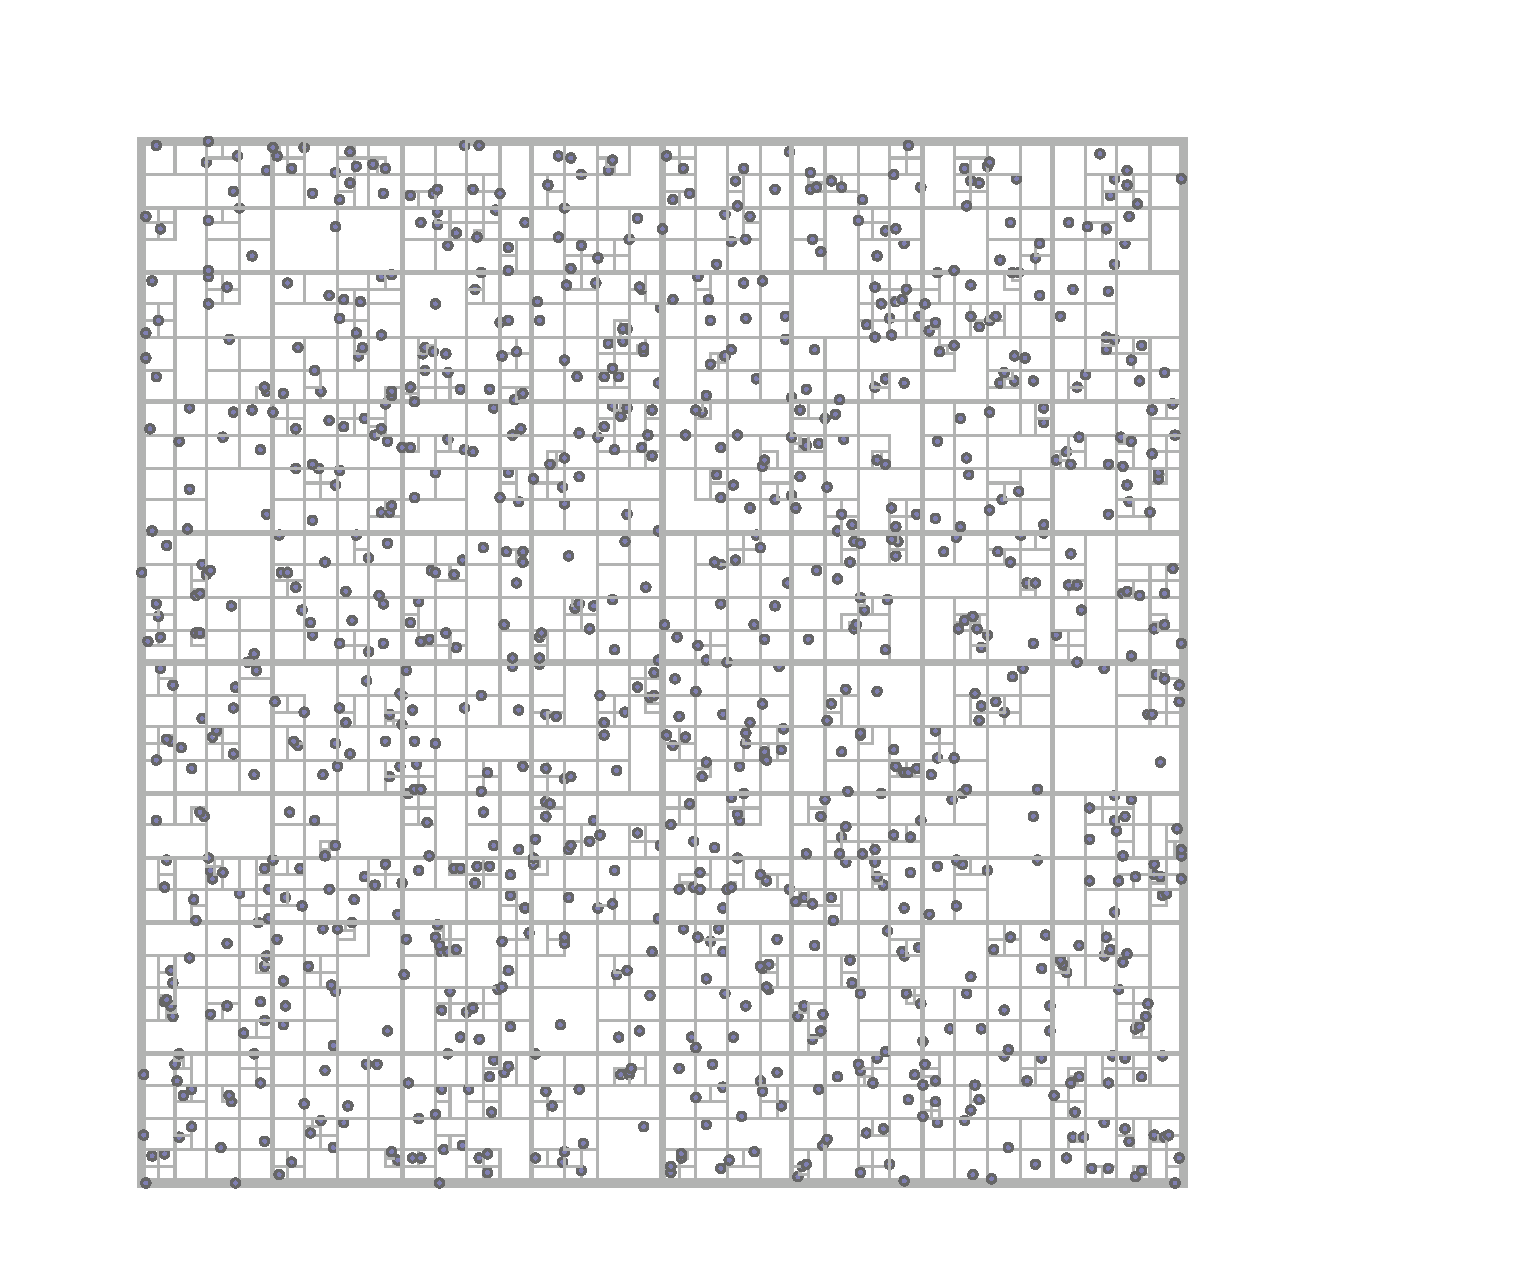
\includegraphics[scale=0.35]{diagrams/quadtree.eps}
\caption{Quadtree}
\end{center}
\end{figure}

Quadtrees can be built over a region, in which case the subdivision proceeds
until the portion of the region covered by a hypercube has the same value for
some property of interest. For example, given an input image, a region based
quadtree would continue to subdivide until each square covered an area which
had the same colour. Quadtrees over a region are called Trie-based quadtrees in
\cite{samet} and can be used to approximate Voronoi diagrams, as discussed
below.

In this section we use quadtrees that are defined over a set of points, in which
case the recursive subdivision is done until each hypercube contains a single
point from the point set.

The root of the quadtree is the hypercube containing all of the points, a leaf
is a hypercube containing a single point, and the height of a quadtree
is the longest path from the root of the quadtree to the leaf of a quadtree
\cite{dutch}.

\begin{thm} \emph{(Height of a Quadtree)}
The height of a quadtree for a set of n points has an upper bound of \(\log(s/c)
+ 3/2\), where c is the smallest distance between any two points in the set, and
s is the side length of the initial square containing all of the points.
\cite{dutch}.
\end{thm}

Note that the height of the quadtree is not bounded by $n$.

\begin{thm} \emph{(Quadtree Construction)}
A quadtree of height h containing n points can be constructed in \(O((h + 1)n)\)
time \cite{dutch}.
\end{thm}

\subsubsection{Point Location in a Quadtree}

Point location in a quadtree is performed by recursively visiting nodes
starting with the root node. At each step, the child node containing the query
point is visited, and the algorithm terminates when a leaf node is reached.

\begin{thm} \emph{(Point Location in a Quadtree)} 
Point location in a quadtree of height h can be performed in time \(O(h)\). 
\end{thm}

\subsubsection{Nearest Neighbour Search in a Quadtree}

Given a query point $p$ the quadtree node containing $p$, if any, can be found by
starting at the root, comparing $p$ to the bounds of the each child of the root,
and recursively visiting the child containing $p$ until a leaf node is found.  
% Fix the remaining missing inline math markup on $n$ and $p$
Since the maximum depth of a quadtree with n points is not bounded by n, the
running time of this search algorithm is also not bounded by n. This search,
along with a means of performing region queries was described in
\cite{quadtree}.

To perform nearest neighbour search in a quadtree we adapt the procedure given
in \cite{samet} for kd-trees. Finding a nearest neighbour in a quadtree is done
by maintaining a priority queue of nodes to visit, which initially contains the
root node. The algorithm proceeds by removing a node from the priority queue and
examining each of its children. If the child node contains a point it is added
to the result set.

Otherwise, the distance from the query point to each child node is calculated
and if it is smaller than the distance to the current furthest result point,
it is added to the priority queue. The work done by this algorithm is at
least the same amount of work required to do perform a point location query.

\begin{thm} \emph{(Nearest Neighbour Search in a Quadtree)} 
Nearest neighbour search in a quadtree of height h requires \(O(h)\) time.
\end{thm}

\subsection{Compressed Quadtrees}

In a compressed quadtree, only nodes which contain a point, or have at least
two child nodes are present in the tree. Compressed quadtrees were first
described in \cite{compressedquadtree}, and a detailed description can be found
in \cite{skipquadtree}.

A compressed quadtree can be created by pruning nodes from an existing quadtree
as follows:

\begin{enumerate}
\item If a node contains no children, remove it.
\item If a node has a single child node, change the pointer to the node in the
node's parent to point to the node's child.
\end{enumerate}

Since this procedure requires first building a regular quadtree, it also
requires \(O((h + 1)n\) time to complete.

This construction procedure can be made more efficient, or at least bounded by
n, by first sorting the points according to Morton (or z-) order. Morton order
is defined by interleaving the bits of each of coordinate of the point, such
that the first bit of the first coordinate is followed by the first bit of the
second coordinate and so on until one bit has been used from each coordinate.
This is then followed by the second bit of the first coordinate \cite{morton}.
When performed in two dimensions, this results in a z-shaped curve. This
interleaving of bits is called the "shuffle" of a point in \cite{bern}.

\begin{figure}
\begin{center}
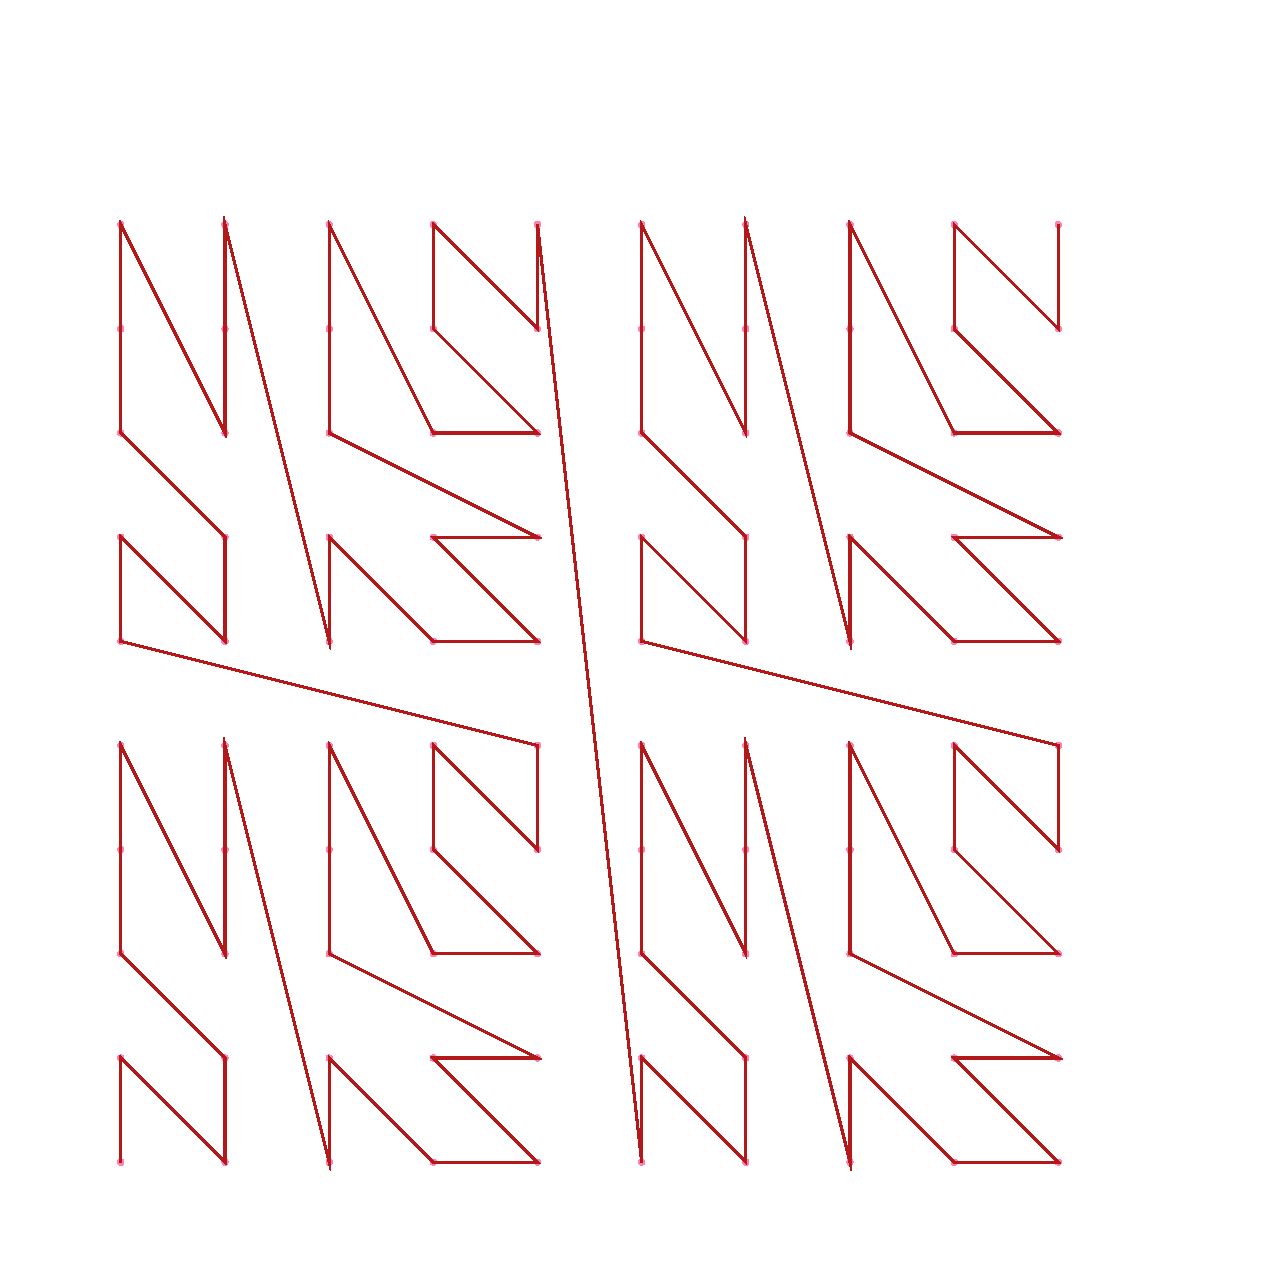
\includegraphics[scale=0.35]{diagrams/zorder.eps}
\caption{Z-Order}
\end{center}
\end{figure}

The points are then sorted according their Morton order. Each two adjacent
points in the sorted order form a node in the quadtree, which can then be
nested by finding the first larger square to the left and the right in the
sorted order \cite{bern}.

\begin{thm} \emph{(Compressed Quadtree Construction)}
A quadtree containing n points can be constructed in \(O(n \log n)\) time
\cite{bern}.
\end{thm}

Chan \cite{chan} showed that the shuffle can be calculated without explicitly
interleaving the bits, and Connor and Kumar \cite{connor} showed that this can be extended from
integer values to IEEE-754 floating point values.

\begin{figure}
\begin{center}
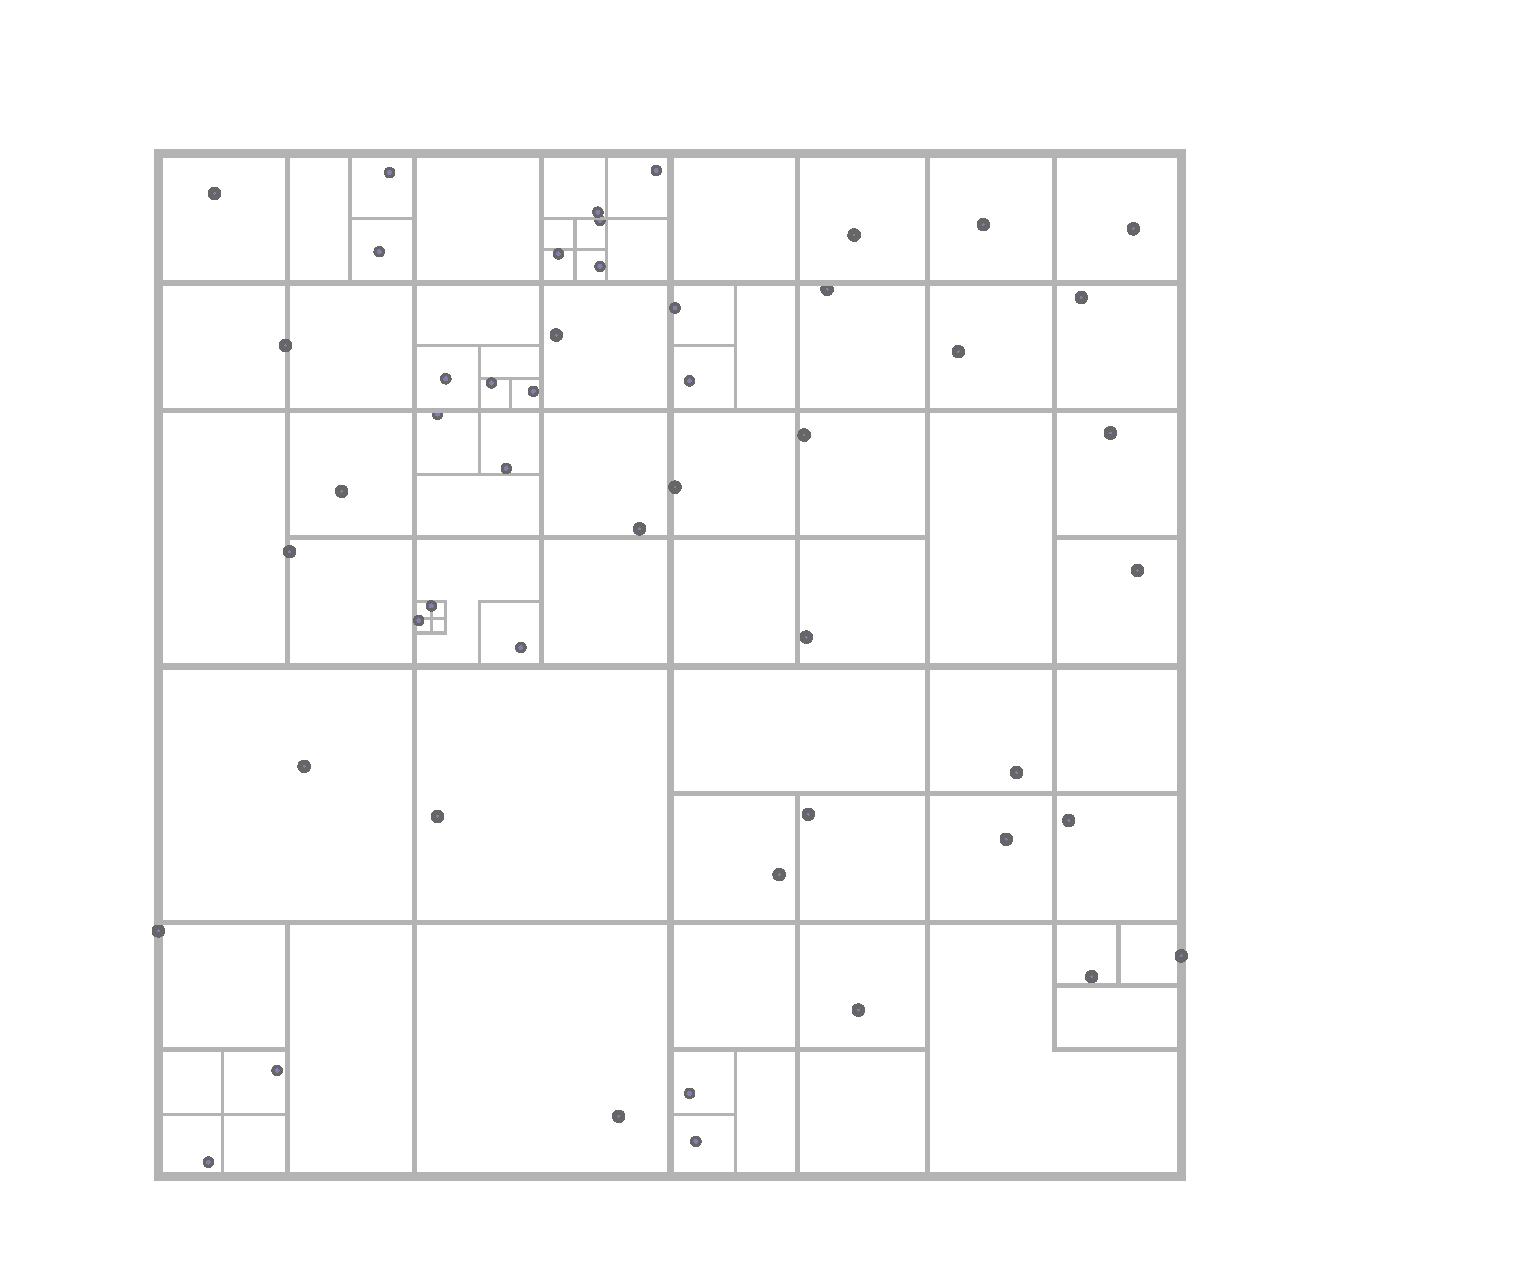
\includegraphics[scale=0.35]{diagrams/compressed_quadtree.eps}
\caption{Compressed Quadtree}
\end{center}
\end{figure}

\begin{thm} \emph{(Height of Compressed Quadtree)}
The height of a compressed quadtree with n points is O(n).
\end{thm}

\subsubsection{Point Location in a Compressed Quadtree}

Point location in a compressed quadtree is done by following the same algorithm
as for standard quadtrees. Since the height of a compressed quadtree is
bounded by the number of points, we can bound the time required to perform
point location.

\begin{thm} \emph{(Point Location in a Compressed Quadtree)} 
Point location in a compressed quadtree with n points can be performed in
time \(O(n)\). 
\end{thm}

\subsubsection{Nearest Neighbour Search in a Compressed Quadtree}

Nearest neighbour search in a compressed quadtree can be done by following the
same algorithm as for standard quadtrees. Again, since the height of a compressed
quadtree is bounded by the number of points, we can bound the time required to
perform point location.

\begin{thm} \emph{(Nearest Neighbour Search in a Compressed Quadtree)} 
Nearest neighbour search in a compressed quadtree with n points requires
\(O(n)\) time.
\end{thm}

\subsection{Skip Quadtrees}

Skip quadtrees extend the idea of skip lists \cite{skiplist} to 2D and higher
dimensional spaces. In a skip list, multiple levels of linked lists exist, with
pointers between the levels.  The bottom level contains all of the nodes, the
top layer is empty, and (in the randomized version of skip lists,) a node
present in a given layer is present in the layer above it with specified
probability.  Corresponding nodes on different levels are then linked. The
expected number of layers is logarithmic, allowing for search in \(O(\log n)\)
time.

Skip quadtrees use essentially the same idea, except each level is a
compressed quadtree rather than a linked list, and terminal nodes in the
compressed quadtree at one level are linked to corresponding nodes in the
lower level tree.  We summarize the results are for the randomized version of
skip quadtrees.  Deterministic results can also be derived using deterministic
skip lists \cite{skipquadtree}.

Since each level of a skip quadtree consists of a compressed quadtree with
approximately half as many points as that in the level below, we expect to
create \(O(\log n)\) compressed quadtrees.

\begin{thm} \emph{(Skip Quadtree Construction)}
% QUESTION: Do you mean to say skip quadtree here?
A quadtree containing n points can be constructed in \(O(n \log^2 n)\)
expected time.
\end{thm}

\subsubsection{Point Location in a Skip Quadtree}

Point location in a skip quadtree is peformed by recursively visiting each level
of the quadtree. Since each level is a compressed quadtree, point location is
first performed in that compressed quadtree. Once the node in the compressed
quadtree is located, the link to the corresponding node in the lower level
is visited until the bottom level is reached and the node in that compressed
quadtree is returned as the result of the point location query. The expected
amount of work performed in each level is constant \cite{skipquadtree}.

\begin{thm} \emph{(Point Location in a Skip Quadtree)} 
Point location in a skip quadtree with n points can be performed in time
\(O(\log n\)) \cite{skipquadtree}. 
\end{thm}

\subsubsection{Nearest Neighbour Search in a Skip Quadtree}

Nearest neighbour search in a skip quadtree is similar to the procedure for
searching a standard quadtree, but the skip structure is used to limit
the number of nodes visited.

% TODO: More math markup around p's and q's
For a node p removed from the priority queue, the skip structure is used to
determine the node q, which is the smallest node in the lowest skip level
which is equidistant to the query point. It is shown in \cite{skipquadtree}
that at most \(O(\log \frac{1}{\epsilon})\) nodes on the path from p to q need
to be added to the priority queue.

\begin{thm} \emph{(Nearest Neighbour Search in a Quadtree)} 
Approximate \(1 + \epsilon\) nearest neighbour search for d dimensions in a skip
quadtree with n points requires
\(O(\epsilon^{1 - d}(\log n + \log \epsilon^(-1)))\) expected time.
\end{thm}

\subsection{Kd-Trees}

Kd-trees were described by Jon Bentley in 1975 as an improvement on quadtrees
\cite{kdtree}.  Kd-trees are binary search trees for which each non-leaf node
divides the point set in half using an axis-aligned line.

Kd-trees are constructed by choosing an axis, determining the median value in
the point set for the corresponding coordinate, and dividing the points in two
halves using the median value.  The two child nodes are then built by
recursively building kd-trees for each half.  Depending upon the application,
a number of heuristics exist for choosing which axis to use for dividing the
points.

FIXME: Actually, Bentley specifies that the discriminators (axes) are chosen roud-robin, level-by-level.

\begin{thm} \emph{(Height of a Kd-Tree)}
The height of a kd-tree with n points is \(O(\log n)\).
\end{thm}

\begin{figure}
\begin{center}
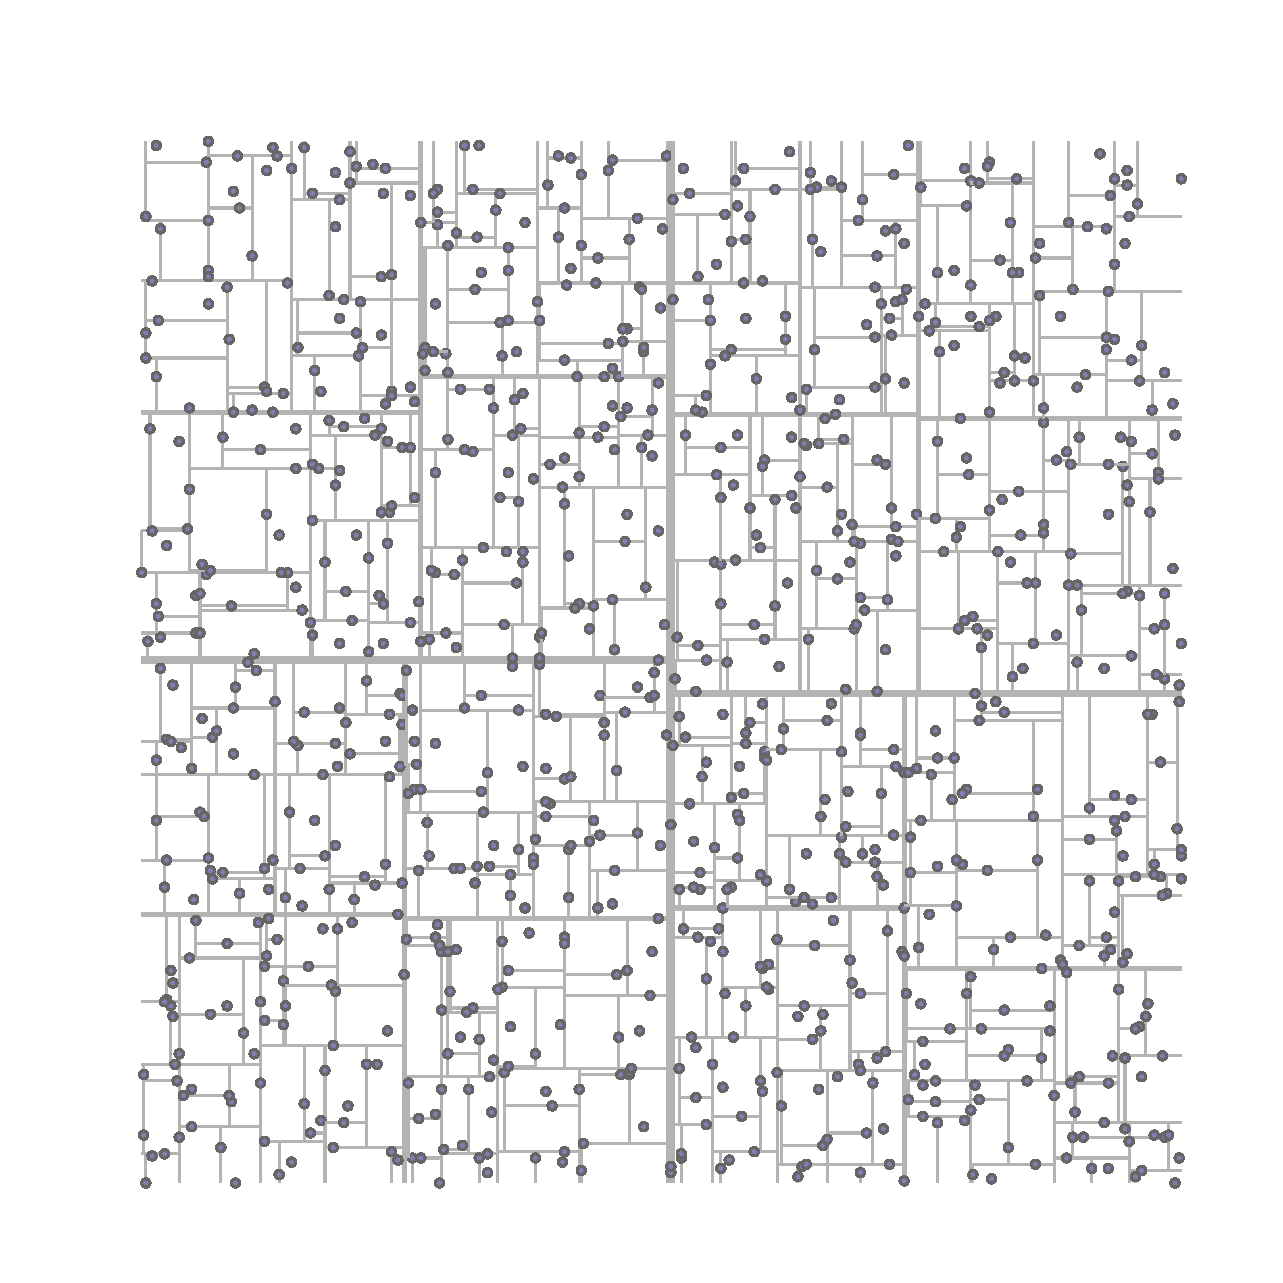
\includegraphics[scale=0.35]{diagrams/kdtree.eps}
\caption{Kd-Tree}
\end{center}
\end{figure}

\subsubsection{Point Location in a Kd-Tree}

Point location in a kd-tree can be performed by recursively visiting nodes and
comparing the appropriate coordinate of the point to the splitting axis used
to split the children for that node, and the visiting the appropriate child
node \cite{kdtree}.

\begin{thm} \emph{(Point Location in a Kd-Tree)} 
Point location in a skip quadtree with n points can be performed in time
\(O(\log n\)). 
\end{thm}

\subsubsection{Nearest Neighbour Search in a Kd-tree}

An algorithm for nearest-neighbour search in a kd-tree tree was described
by Friedman et al. \cite{friedman} in 1977 as an improvement on the algorithm
contained in the original paper describing kd-trees.

The algorithm proceeds in a manner similar to the procedure for point-location,
but at each step the child node that was not visited is added to a priority
queue. When a leaf node is reached, the point at that node is added to the
result set and the priority queue is examined. If the closest node in the
priority queue is closer than the furthest point in the result set, then it
is visited according to the recursive procedure given for point location. 

For a \(1 + \epsilon\) approximate nearest neighbour search, nodes in the
priority queue are only visited if they closer than \(1 + \epsilon\) times
the distance to furthest point in the result set.

\begin{thm} \emph{(Nearest Neighbour Search in a Kd-tree)} 
The expected time for nearest-neighbour search in a kd-tree with n points is
\(O \log(n)\), and the worst case is \(O(n)\) \cite{friedman}.
\end{thm}

\subsection{Balanced Box Decomposition (BBD) Trees}

A balanced box decomposition tree is a data structure invented by Arya et al.
\cite{optimalann} which combines advantages of both quadtrees and kd-trees.
Like a kd-tree, as one traverses the tree, the number of points decreases
exponentially, and like a quadtree, the area also decreases exponentially. By
combinging these properties, an optimal data structure for approximate nearest
neighbour search is obtained.

Each node in a BBD-tree covers a cell which is the set theoretic difference
between an outer box and an optional inner box. Both boxes are axis-aligned.
If present, the inner box must either touch the edge of the outer box, or be
separated from each edge by at least the width of the box in the direction of
the edge. Each node is an BBD-tree has a bounded aspect ratio which ensures
that the ratio of the shortest edge to the longest edge is bounded by some
constant.

A BBD-tree is constructed through a sequence of two operations, fair-splits
and shrinks. A fair-split is a partition of a box using an axis aligned
hyperplane, which maintains the aspect ratio bound but does not necessarily
result in an even partition of points. A shrink operation divides a node into
inner and outer boxes, which is used in a manner similar to a compressed
quadtree, and can ensure an even partition of points \cite{optimalann}.

Both fair-splits and shrinks can be performed in time linear in the number of
points contained in the cell. A simple strategy for partitioning the points is
the midpoint algorithm, which performs a fair-split by partitioning the node
with a hyperplane orthogonal to the longest edge of the outer box. A shrink
operation is somewhat more complicated, potentially requiring two shrink nodes
and one split node to ensure that no child contains more than \(2/3\) of the
points covered by the parent node \cite{optimalann}.

To prove properties of the BBD-tree, Arya et al. assume that fair-splits and
shrinks are applied alternately as the tree is constructed. In practice, they
note that for almost all cases, only fair-splits are required \cite{optimalann}. 

\begin{thm} \emph{(BBD-Tree Construction)} 
A BBD-tree for a \(d\)-dimensional space has \(O(n)\) nodes and can be build in
\(O(d n \log n)\) time \cite{optimalann}.
\end{thm}

\subsubsection{Nearest Neighbour Search in a BBD Tree}

Nearest neighbour search in a BBD Tree is performed in a manner similar to
search in a kd-tree. A priority queue is maintained of nodes to visit which
initially contains the root node. At each step of the search, the closest
node to the point is removed from the queue and is recursively searched for
the leaf closest to the search point. The distance to the other child nodes
encountered in the search is calculated and they are enqueued in the priority
queue. The search continues until the distance to the node at the top of the
priority queue exceeds the distance to the candidate nearest neighbour. This
can be easily extended to find k nearest neighbours, and to find approximate
nearest neighbours rather than an exact ones.

\begin{thm} \emph{(Nearest Neighbour Search in a BBD Tree)} 
Given a constant \(c_{d,\epsilon} \le \lceil 1 + {6d \over \epsilon} \rceil^d\)
where d is the dimensionality of the space and \(\epsilon\) is the approximation
factor, a \((1 + \epsilon)\)-nearest neighbour search in a BBD Tree can be
performed in time \(O(c_{d,\epsilon} \log n)\) time and k approximate nearest
neigbhours can be found in \(O((c_{d,\epsilon} + kd) \log n)\) time.
\end{thm}

\subsection{Approximate Voronoi Diagrams}

For approximate nearest-neighbour searches, it is possible to improve on the
space requirements by creating an approximation to the Voronoi diagram, for
instance using quadtrees \cite{avd}. The complexity of the calculation is
reduced by constructing the Voronoi diagram such that for each cell, any point
within it is a \(1 + \epsilon\)-nearest neighbour, rather than an exact
nearest neigbhour.

Har-Peled \cite{avd} provides an algorithm for building an approximate
Voronoi diagram which that answers nearest-neighbour searches. His
construction is complicated, requiring first clustering the input sites, then
building a data structure for answerings point location in equal ball queries
(a technique also used in locality sensitive hashing \cite{lsh}) and finally
using this data structure to build the approximate Voronoi diagram using
compressed quadtrees.

Arya et al. \cite{arya-avd} extend this to \(t, \epsilon\)-AVD where each
cell in the approximate Voronoi diagram stores \(t\) approximate nearest
neighbours. Their construction makes use of a well-separated pair
decomposition of the sites of the Voronoi diagram. Two sets of points are well
separated if each set can be bounded by a ball of radius \(r\) such that the
distance between the center of each set is at least \(2r\). By decomposing
the sites into well-separated subsets, a set of quadtree nodes can be
generated which are then stored in a BBD-tree. 

We do not describe the construction algorithm in detail as these results are
not used in the remainder of the thesis. We note that both \(\epsilon\) and t
need to be fixed at construction time, which is a less flexible than using
quadtrees or kd-trees directly.

\begin{thm} \emph{(Nearest Neighbour Search in a Approximate Voronoi Diagram)} 
An approximate Voronoi diagram of size \(O({n \over \epsilon ^ d})\) can be
constructed which can answer \((1 + \epsilon)\) approximate nearest neighbour
searches in time \(O(\log {n \over \epsilon})\) \cite{arya-avd}.
\end{thm}

% TODO: give further justification for not considering AVD more seriously
% (too complicated? unimplementable? ...)

\section{Biased Search}

In this section we examine biased search problem in a comparison tree model.
The comparison tree model is suitable for geometric problems as it avoids
numerical and geometrical robustness problems that can arise from computations
using coordinates.  We begin with some classical results for biased search trees
in a single dimension, before considering the problem in higher dimensional spaces.

\subsection{Information Theory}

Lower bounds for search, in particular biased search, depend upon results from
information theory. We briefly summarize these results here.  Information theory
is the study of the fundamental properties of communication systems. A data
structure can be seen as a form of communication system, since it provides a
means of communicating data from the present to the future.  A data structure
which allows for efficient search is essentially solving the same problem as
creating an efficient code with which to transmit a message.

Based upon earlier work by Ralph Hartley, Claude Shannon \cite{claudeshannonwasagod}
defined entropy as the measure (in bits) of the amount of randomness of a set.
That is if \(p_i\) is the probability of the i-th member of the set, then the
entropy \(H\) is defined as
$$
H = \sum{ p_i \log{1 \over p_i}}
$$

Shannon also proved that the efficiency of any communication system is limited
by the entropy of the set of messages to be transmitted.

\begin{thm} \emph{(Fundamental Theorem for a Noiseless Channel)} 
Given a source with entropy H (in bits) and a channel with capacity C (in bits
per second), then it is possible to encode a source in such a way as to
transmit at an average rate of \({C \over H} - \epsilon\) symbols per second
where \(\epsilon\) is arbitrarily small, and it is not possible to transmit
at an average rate greater than \(C \over H\) \cite{claudeshannonwasagod}.
\end{thm}

Any data structure for search can not have an expected average search time which
exceeds this entropy bound, that is \(\Omega(H)\) is a lower bound on the search time
for any data structure.

% Emphasize somewhere, early on, that "search time" = "# comparisons"

% This is critical, and needs to be elaborated on.
% You say that Omega(H) is a lower-bound, but H is defined in terms of p_i's,
% so you also have to say what those are.  Also specify that this is for a
% random query where the data structure has no information about this query
% other than the distribution of its outcomes

\subsection{Biased Search Trees}

Biased search trees are a natural generalization of balancing a binary search
tree where rather than assuming each result is equally likely, a probability
distribution (or set of weights) is given for the results, allowing the tree to
be balanced such that at each node the probability of choosing the right child
is as close as possible to the probability of choosing the left child, or
alternately, the weight of the right child is approximately equal to the weight
of the left child.

The initial work on biased search trees focused on the static case, where
the query frequencies are known in advance and no deletions and insertions
are allowed. This work is summarized in Volume 3 of the Art of Computer
Programming \cite{knuth}.

Given a set of n keys \(K_i\) and \(2n + 1\) probabilities
\(p_1, p_2, ..., p_n\) and \(q_1, q_2, ..., q_n\) where \(p_i\) is the
probability that \(K_i\) is the search item and \(q_i\) is the
probability that the search item lies between \(K_i\) and \(K_{i+1}\), an
optimal biased search tree is one that minimizes the expected number of
comparisons to search the tree \cite{knuth}.

Each subtree of a optimal biased search tree is itself optimal, and so the
problem can be solved through a dynamic programming algorithm, using the
following relation: Define \( c(i,j)\) as the cost of an optimum subtree with
weights \((p_{i+1}, ..., p_j; q_{i+1}, ..., q_j;)\) and \(w(i, j)\) be the
sum of the weights, i.e. \(p_{i+1} + ... + p_j + q_{i + 1} + ... + q_j \)
\cite{knuth}.

Then we have that:

\begin{equation}
    \begin{aligned}
    c(i, i) & = 0 \\
    c(i, j) & = w(i, j) + \min_{1<k<j} (c(i, k - 1) + c(k, j)), \text{for } i<j, \\
    \end{aligned}
\end{equation}

This recurrence allows us to find all optimal one node trees and then use that
to find all optimal two node trees, and so forth, until an optimal search
tree has been determined. This minimization is applied to \({1\over{6}} n^{3} \)
values of \( k \), but an monotonicity property allows the running time
to be reduced to \( O(n^2) \) \cite{knuth}.

\begin{thm} \emph{(Construction of an Optimal Static Biased Binary Search Tree)} 
An optimal static biased search tree can be constructed in time \(O(n^2)\) and
space \(O(n^2)\) using a dynamic programming approach \cite{knuth}.
\end{thm}

Knuth also proposed two heuristics which run in \(O(n \log n)\) time and
\(O(n)\) space which produce nearly optimal trees:

Rule I: Use the most frequent item as the root of the tree and apply the same
rule to the subtrees.

Rule II: Choose as the root the item which results in the weight of the left
and right subtrees being as close to equal as possible and apply the same
rule to the subtrees. 

Mehlhorn \cite{mehlhorn} analyzed the results of applying these two rules. He
provides a simple example where Rule I will produce a tree with expected
search time \(\Theta(n)\).

His analysis of Rule II shows that the expected search time for item in the tree
is bounded from above by the entropy \(H\) of the query frequency distribution.
That is, if we have n keys \(K_i\) and \(2n + 1\) probabilities
\(p_1, p_2, ..., p_n\) and \(q_1, q_2, ..., q_n\) where \(p_i\) is the
probability that \(K_i\) is the search item and \(q_i\) is the
probability that the search item lies between \(K_i\) and \(K_{i+1}\), then
the search time is bounded by
$$
H = \sum{ p_i \log{1 \over p_i}} + \sum{ q_i \log{1 \over q_i}}
$$

% FIXME: Look at Mehlhorn's paper again.  There is, I believe an O(1) term

\begin{thm} \emph{(Nearly Optimal Static Biased Binary Search Tree)} 
A static biased search tree where the search time for an item is bounded by
the entropy \(H\) of the frequency distribution can be constructed in time
\(O(n \log n)\) and space \(O(n)\).
\end{thm}

Biased search trees allowing insertions and deletions based upon 2-4 and
red-black trees were described by Bent, Sleator and Tarjan \cite{bst} in 1984.
As with 2-4 trees, their data structure relies upon maintaing invariants
on the tree during updates through complicated, multi-case rules for
re-parenting nodes to maintain balance. In this case, the balance condition
depends upon the weight of the node. If all of the weights are one, the
resulting tree is simply a 2-4 tree. Somewhat simpler trees are provided
by Feigenbaum and Tarjan \cite{bst2}. Due to the complexity and number of
sub-cases that must be considered to maintain balance in the search tree, we do
not provide further implementation details.

\begin{thm} \emph{(Construction of a Dynamic Biased Binary Search Tree)} 
A dynamic biased search tree can be constructed in time \(O(n)\) which can
perform searches in time \(O(\log(w))\) where \(w\) is the weight of the item
searched for and insertions and deletions in ammortized time \(O(W / w)\)
where \(W\) is the total weight of all items in the search tree and \(w\) is
the weight of the item added or removed \cite{bst2}.
\end{thm}

\subsection{Splay Trees}

An alternative approach to biased search is to use data structures which
modify themselves in response to queries. In this case, rather than specifying
the probabilities in advance, the data structure will change itself to match
the query distribution. 

Splay trees, which were invented by Sleator and Tarjan \cite{splaytree} are a
self-modifying binary search tree which perform well in practice. They operate
by moving the most recently accessed node to the root of the tree using a
process called splaying which rotates items in pairs according to three cases
which depend upon the structure of the tree.

Although splaying can be costly for an individual access, in an ammortized
sense, operations on a splay tree take \(O(\log n)\) time.

\begin{thm} \emph{(Splay Trees)} 
Insertion, deletion and search in a splay tree take \(O(\log n)\) time in
an ammortized sense \cite{splaytree}.
\end{thm}

Sleator and Tarjan also showed that splay trees perform within a constant
factor of any static optimal search tree over a sequence of accesses, and
famously, conjectured that splay trees also perform within a constant factor
of any dynamic search tree as well.

\begin{thm} \emph{(Static Optimality of Splay Trees)} 
The total ammortized time required for a sequence of \(m\) accesses to a \(n\)
node splay tree is \(O(n \log n + m)\) \cite{splaytree}.
\end{thm}

It is possible to create biased versions of other, simpler data structures
such as randomized search trees (treaps) \cite{treap} and skip lists
\cite{bsl2} but these do not provide better theoretical performance guarantees
than biased search trees. In practice, splay trees appear to have better
performance and are as easy to implement as treaps and skip lists, and so these
data structures are not discussed further \cite{minor}.

\subsection{Planar Point Location}

Looking at biased search in higher dimensions, we first consider the planar
point location problem, which is, given a subdivision of the plane and a
query point \(p\), construct a data structure which allows us to efficiently
determine which face of the plane contains \(p\). If all of the planar
subdivisions and the query point lie on a single line then this problem is the
traditional one dimensional search problem, and the appropriate data structure
is a binary search tree.

We discussed this problem above in the section on nearest-neighbour
search in a Voronoi diagram, and noted that a linear space and \(O(\log n)\)
search time solution existed for this problem.  
%% Be more precise here: p_i is the probability that the _answer_ to a query
%% is the i'th triangle
FIXME: As is the case with binary
search trees, if we are given a probability distribution over the query points
\(p\) such that each point is chosen with probability \(p_i\), then the
expected number of decisions made during search is bounded by the entropy of
the query set.

A data structure for biased point location in a triangulation was described
by Iacono \cite{iacono}. It is based on a variation of Kirkpatrick's data
structure for solving point location \cite{kirkpatrick}, which works by
constructed a hierarchical triangulation by selectively removing vertices
from each level of the hierarchy, until the top level contains a single triangle.
In Iacono's version, the vertices chosen to be removed are such that they are
not of large degree and are not incident to a high probability region. Another
approach, by Arya et al. matches these space and time bounds \cite{simpleentropy}.

\begin{thm} \emph{(Distribution Sensitive Point Location in a Triangulation)} 
Given a triangulation, it is possible to perform point location in time
\(O(H + 1)\) and space \(O(n)\) where H is the entropy of the set of triangles
making up the triangulation. 
\end{thm}

\subsection{Biased Range Search}

We next consider results by Dujmovic et al. \cite{biasedrange} on 2-sided
planar orthogonal range counting Range counting is the problem of counting the
number of elements in a set \(S\) contained within a query space. The 2-sided
orthogonal planar variant restricts this to counting the number of elements
\((p_x, p_y)\) given a query point \((q_x, q_y)\) where \(p_x \ge q_x\) and
\(p_y \ge q_y\). Although this is a restricted problem definition, the approach
taken is similar to that used by Odds-on Trees to solve more general geometric 
search problems.

A data structure invented by Jon Bentley \cite{rangetree} called a Range Tree
can solve range search problems in linear space and logarithmic time. A one
dimensional range tree is simply a balanced binary search tree, and in \(d\)
dimensions, one coordinate is chosen to create a binary search tree, and each
child node contains a \(d - 1\) range tree. 

\begin{thm} \emph{(Planar Range Search using Range Trees)} 
A range tree for a set of points \(S\) of cardinality \(n\) can be built in
time \(O(n \log n)\) and requires \(O(n \log n)\) space. It can report the
points in a rectangular query area in time \(O(\log^2 n + k)\) time, where
\(k\) is the number of points in the query area. A technique called
fractional cascading can reduce the query time to \(O(\log n + k)\)
\cite{dutch}. 
\end{thm}

Kd-Trees and Quadtrees can also be used to solve the range counting problem,
but with linear worst case query time.
% Actually, kd-trees can answer orthogonal range counting queries in $O(\sqrt(n))$ time per query.


% In this section, it would be good to give an example of the
% entropy argument.  The answer to any range counting query is an
% integer in {0,...,n}.  p_i is the probability that the answer is i.
% Then H=\sum_{i=0}^n{p_i\log(1/p_i) is a lower-bound.

% Then you can show an example like like Figure~1.b in \cite{biasedrange}
% that shows that H can be big even if the query distribution is such that
% the answer to a range counting query is always 0.


A Biased Range Tree relies upon two data structures. The primary search tree
is based upon a kd-tree. The nodes of the primary tree are associated with
regions of space, and the root node covers the plane. Any node in the primary
search tree that has depth greater than \(O(\log n)\) is called a ``bad'' node.
These regions are potentially open on two sides, since the data structure is
designed to support 2-sided queries \cite{biasedrange}. 

Each child node in the tree is constructed by removing a horizontal (at even
depths) or vertical (at odd depths) strip from region associated with the
parent region. These strips are constructed such that the probability a point
being in the region associated with a child node is at most half the probability
of the point being in the parent region.

Each node also has two associated data structures, called catalogues, which
contain subsets of \(S\) sorted by the x- and y- coordinates respectively.
Each catalogue is indexed by a biased search tree, and fractional cascading is
used to speed up search within the catalogues.

The second data structure is a backup range tree, as described above, which
uses \(O(n \log n)\) space and can answer range search queries in time
\(O(\log n)\). This data structure is used to answer queries for which the
depth of corresponding node in the primary tree would exceed \(O(\log n)\),
that is the "bad" nodes.

Search within the biased range tree occurs as follows: the primary tree is
first searched to find a node such that the query region defined by \(q_x\) and
\(q_y\) is contained within the region corresponding to the node. If this node
is a "bad" node, then the backup range tree is used to answer the query.
Otherwise, the indices are used to locate the node are used to locate \(q_x\)
and \(q_y\) in the catalogues for the node determine the result of the range
counting query, and the tree is walked back to the root, locating the query
point in the catalogues of each node along the way, and adding results to
the range counting query.

% The definition of H needs to be fixed here.  H is a function of the points
% and query distribution that lower-bounds the expected number of comparisons
% done by any comparison-based data structure 

\begin{thm} \emph{(Two-Sided Orthogonal Biased Range Search)} 
Two sided orthogonal biased range search can be performed using space
\(O(\log n\)) and expected time \(O(H)\) where \(H\) is the entropy of the query
set \cite{biasedrange}.
\end{thm}


\subsection{Odds-on Trees}

Odds-on trees make use of similar ideas of those described above to solve
2-sided orthogonal range searches, but are capable of solving a large class
of geometric search problems.

Given a probability distribution \(D\) over a set of queries, the odds-on tree
is capable of answering any query drawn from \(D\) in expected time
\(O(H^* + 1)\) where \(H^*\) is a lower bound on the expected cost of any
linear decision tree which solves the search problem. In particular, the
entropy \(H\) of the query distribution \(D\) is one such bound for many search
problems.
% Again, it's the entropy of the ouput that matters, not the entropy of the 
% query distribution (which may not even be well-defined).
A linear decision tree is a search tree where the decision of which
child node to follow is based on a linear function.

An Odds-on tree consists of a primary search tree and a backup search tree.
The primary search tree is based upon a data structure called partition trees,
which are an means of dividing \(d\)-dimensional spaces into simplices. A
simplex is the intersection of at most \(d + 1\) halfspaces; a triangle is an
example of a simplex in two dimensions. The simplices in the partition tree
potentially overlap each other.

\begin{thm} \emph{(Partition Trees)} 
Given a set of \(S\) points, for any \(\epsilon > 0\) a data structure called
a partition tree can be constructed which uses \(O(n)\) storage and can answer
counting queries for a search simplex in time \(O(n^{1/2 + \epsilon})\) time and
report those points in an additional \(O(k)\) time, where \(k\) is the number
of points in the search simplex. A partition tree can be constructed in
\(O(n^{1 + \epsilon})\) time \cite{dutch}.
\end{thm}

The points used to create this partition are drawn from the query distribution
\(D\), and the maximum depth of any node in the tree does not exceed a specified
constant. For each node in the partition tree the area corresponding to the node
is searched to see if the answer to the search problem is the same for all points
associated with the area. Since the simplices created by a partition tree are
possibly overlapping, it is necessary to determine the polytope associated with
the node which is not associated with any other node in the tree.

If the result of the search is the same for all points in the polytope, the node
is marked as terminal, any children nodes are removed, and the result of the
search is stored with the node to answer future searches.

The backup tree can be any data structure capable of answering the original
search problem in \(O(\log n)\) time.

Search in the tree occurs as follows. Given a query, the tree is searched until
either a terminal leaf node is reached, in which case the stored result is used
to answer a query, or a non-terminal leaf node is reached, in which case the
backup tree is used to answer the query \cite{oddson}. The same data structure
with a different analysis was presented by Chan et al. \cite{chan}.

\begin{thm} \emph{(Odds-on Tree)}
For any \(n\) and \(\tau>0\) an odds-on tree of size \(m = n^\tau\) of maximum
depth k = \(\lfloor {1 \over 4} \log_{r \over 3} m \rfloor \), where \(r\) is
the number of simplices associated with the root node of the odds-on tree, can
be constructed in time \(O(m \log^{O(1)} n)\) plus the cost of \(O(m)\) samples
from \(D\) plus the cost of \(O(m \log^{O(1)} n)\) searches to determine whether
a node is terminal.

The odds-on tree can be answer searches in expected time \(O(H^* + 1)\) where
\(H^*\) is a lower bound on the expected cost of any linear decision tree
which answers the search \cite{oddson}.  
\end{thm}

\chapter{Implementation}

This chapter describes the implementation of the odds-on tree data structure
for nearest-neighbour search.

The theoretical properties of odds-on trees were derived using partition trees.
Partition trees are a complicated data structure and to our knowledge, have
never been implemented. Although compressed quadtrees and kd-trees lack strong
theoretical performance guarantees, they have the advantage that they are
simple to implement and perform well in practice.

In general, kd-trees out perform quadtrees, but we chose to implement both data
structures to see if building a compressed quadtree ``bottom up'' using z-order
sorting would result either in faster construction time or faster query time
than a traditional ``top down'' recursive build process.

\section{Kd-tree Odds-on Tree Implementation}

This section describes the implementation of kd-trees and the kd-tree based
odds-on tree implementation.

\subsection{Kd-tree Implementation}

We first describe the kd-tree implementation. The kd-tree is built as described
in chapter two, by recursively splitting the point set along each axis.  A lot
of work has been done on heuristics for choosing which axis to split along when
constructing kd-trees, particularly in the computer graphics community where
kd-trees are used to accelerate ray tracing applications
\cite{physicallybasedrendering}.

We choose to use the naive approach of splitting along each axis in sequence.
In our experimental work, we are comparing the performance of the odds-on tree
to same kd-tree implementation used by the odds-on tree, so any performance
gains would most likely be realized by both data structures and so would not
impact the experimental results.

TODO: This might actually be interesting to investigate in the experimentation.
A better partitioning strategy could potentially build a better odds-on tree,
or at least build a good one more quickly.

The most significant optimization made during the implementation is to use
a memory pool rather than the system allocator for allocations. This allowed
for left and right children of a node to be placed at adjacent locations in
memory for better locality of reference and avoided the overhead associated
with many small allocations using the system allocator, which resulting in a
50 percent improvement in running time. The implementation was based upon the
kd-tree optimization notes in \cite{physicallybasedrendering}.

In order to support odds-on tree construction, the construction routines in
the kd-tree were modified to optionally support making a callback function
call as each node is constructed. If the callback returns false, the kd-tree
construction ends without processing all of the points. This callback
mechanism also allows for additional information to be stored at the kd-tree
node if it is so desired.

We performed some experiments comparing our kd-tree implementation to the 
kd-tree implementation in Mount and Arya's ANN library\cite{ann}. Our
implementation was slower, but not by a large amount. For instance, running
1000000 queries on a point set of 100000 points, our implementation was eleven
percent slower in two dimensions and eighteen percent slower in three
dimensions.

\subsection{Odds-on Tree Implementation}

The odds-on tree is built using two point sets. The first point set is used
to build the backup kd-tree which is used to answer queries which can not be
efficiently answered using the odds-on tree, and during construction to
determine if a newly constructed node.

The second point set is a set of points drawn from the probability distribution
describing query frequencies, and is also used to build a kd-tree. This build
process takes advantage of the callback functionality to stop building the
kd-tree if it can be determined that the answer to a nearest-neighbour query
would be the same for all points covered by the node, which is done by
running a nearest neighbour query for each of the "corner" points of the node.
If each query returns the same nearest neighbour point, the node is marked
as terminal and the nearest neighbour is stored with the node.

A maximum depth for a constructed node is also enforced by the callback
function which will end the build process for a node without marking it
terminal if the depth of its subtree will exceed a pre-determined maximum.

The build process continues until one of three conditons occurs: all input nodes
have been processed, all nodes have been marked terminal, or all remaining nodes
exceed the maximum depth specified.

\section{Quadtree Odds-on Tree Implementation}

The Quadtree based odds-on tree is implemented using compressed quadtrees.
Initially, the compressed quadtrees were based upon sorting by Morton order.
This was found to not perform well, and a second implemention, based upon top
down recursive construction is now used.

\subsection{Morton Order Implementation}

The compressed quadtree data structure used by the odds-on tree was first
implemented using Morton order based sorting. As described in section 2.1.3,
points sorted by Morton order are sorted in the order in which they would be
visited during a depth first traversal of a compressed quadtree.

The sorted points were then visited in order to find sequences of points with
a common nearest neigbhour. Once a sequence was discovered, the end points
were used to construct a bounding box, and the "corners" of the bounding box
were tested using a backup kd-tree structure. If all of the corners shared a
common nearest-neigbhour, the bounding box is marked as terminal and added to
a list of cache nodes.

After all of the sorted points have been processed, adjacent nodes in the list
of cache nodes are used to build a bounding volume hierarchy which is used as
the cache for the odds-on tree.

Both minimal (i.e. two point) and maximum sequences were tested to see which
would perform better when constructing the tree. Maximal sequences result in
smaller cache structures, but correspondingly worse cache hit rates. Neither
implementation is competitive with kd-trees, and so the Morton order based
implementation was replaced with a compressed quadtree based implementation.

\subsection{Compressed Quadtree Implementation}

The compressed quadtree is built from the top down through recursive calls to a
build function. The root node is covers the area containing all of the input
points, and each node is split in to \(2^d\) equal size children. The build
procedure is then called recursively for each child. Once the children are
built, the node is examined to see if it only contains one child node. If so,
the node is removed and the child node is returned in its place, which causes
a compressed quadtree to be built.

As with the kd-tree based implementation, a callback function is called as
each node is created, which allows for the build process to end before all
nodes are processed.

The odds-on tree itself is built using a similar process to the kd-tree based
version, using two point sets. The first point set is used to build a backup
kd-tree, and the second set is used to build the compressed quadtree which
is used as the cache. The interference query procedure is identical with the
version used in the kd-tree based odds-on tree. A maximum depth is enforced.

Building the compressed quadtree implementation top down was not as fast as
sorting by Morton order, but resulted in a higher quality cache, so that cache
hit rates were higher, and overall performance was better.

TODO: give some figures comparing build times and query times between versions.

\section{Odds-on Tree Query algorithm}

The query algorithm is handled in a similar fashion by both the kd-tree and
quadtree based implementions, and is described in this section.

Both implementations rely upon a locate procedure which searches the cache for a
terminal node containing the query point. If only a single nearest neighbour
is required, if such a terminal node exists, the cached value for nearest
neighbour is returned; otherwise, the backup cache is searched for the
nearest neighbour.

If k nearest neighbours are required, it is always necessary to use the the
backup cache. In this case, the locate procedure is used as above, but as it
proceeds, each node visited is stored in a priority queue which is then passed
into the backup node. This is used to prune the search while locating the true
k nearest neighbours, which in favourable conditions can greatly accelerate
the search process.

\chapter{Experimental Results}

\section{Experiment Design}

The experimental hypothesis is that the odds-on tree provides better k-nn
performance than a kd-tree implementation in cases where the entropy of the
query set is sufficiently low.

This hypothesis is tested using both synthetic data drawn from probability
distributions, and with data derived from applications of nearest neighbour
search. 

\subsection{Synthetic Data}

\subsubsection{Implementation}

Since preliminary experimentation with the kd-tree and quadtree based
implementations did not show one to out perform the other consistently, each
experiment was repeated for both implementations.

\subsubsection{Dimension}

TODO:
- will definitely experiment in 2, 3, 4 dimensions.
- both kd-trees and quadtrees perform poorly in higher dimensions.  The "curse
of dimensionality" says the number of sample points required to build the cache
should grow quickly as dimension increases, but kd-tree performance also quickly
gets worse.
- will try 8, 16 dimensions in a limited number of cases to see if it is worth
while doing full studies, but literature says this will likely not work well.

\subsubsection{Point Set}

The point set

- distribution of points: uniform or mixture of gaussians
- number of points: 10000, 100000, 1000000 

To reduce variance, the point set which was queried to determine the nearest
neighbour was maintained between trials.  Two distributions were used for the

\subsubsection{Sample Set}

The sample set is the set of searches used to build the odds-on tree.

\subsubsection{Search Set}

The search set is the set of searches used to  test the odds-on tree and
kd-tree implementations.  In all cases, the search set is drawn from the same
distribution used to generate the sample set, and the number of searches was
fixed at 1000000. 

TODO: briefly describe distributions used to generate points: uniform, gaussian,
mixture of gaussians.

\subsection{Application Data}

Sites such as ColorLovers.com \cite{colorlovers} allow users to define a
colours as a triplet of RGB values, which are used in turn to define colour
themes, which are sets of 1 or more colours which work well together in a
design.

One may want to find the nearest named colour to a given RGB value for
a number of reasons, including buying a paint formulation which matches the
desired colour.  For instance, ColorLovers will provided the closest Martha
Stewart paint colour to a given colour if a user wishes to use a paint.

In the Pantone \cite{pantone} printing process, colours are chosen from a set of
approximately 1000 spot colours rather than using mixtures of four inks as is
done in the CMYK process.

Since some colours are more popular choices than others, in particular when
creating colour themes, this provides a biased search in three dimensions. We
use the colour theme datasets created by \cite{colorthemes}.

\section{Measuring Performance}

\subsection{Benchmark Platform}

An Intel Core I5 laptop was used as the benchmark platform.

\subsection{Performance Metrics}

The primary performance metric is running time.  For each experiment
configuration, 1000000 queries are performed and the elapsed system clock
time is recorded.

In addition to running time, data is collected on the cache miss rate for the
odds-on tree, as well as the number of nodes visited in both the cache and the
back up tree.

Since cache utilization can have a major impact on running time, the Valgrind
\cite{valgrind} cachegrind utility is used to simulate the cache performance
of the implementation, and data is collected on L1 and L2 cache miss rates.

\section{Results}

TODO: one section for each experimental configuration.

\chapter{Conclusion}

\section{Summary}

TODO:

\section{Future Work}

TODO:

\begin{thebibliography}{5}

\bibitem{treap}
Aragon, C. R.,  Seidel, R. (1996) Randomized Search Trees.
In Algorithmica, Vol. 16, Number 4/5, pp. 464--497

\bibitem{fastvector}
Arya, S., Mount, D. M. (1993) Algorithms for Fast Vector Quantization,
Proceedings of DCC '93, IEEE Press, pp 381--390. 

\bibitem{app-ann}
Arya, S., Mount, D. M. (1993) Approximate nearest neighbour queries in Fixed
Dimensions, Proceedings of the 4th ACIM-SIAM Symposium on Discrete Algorithms,
pp 271 -- 280.

\bibitem{optimalann}
Arya, S., Mount, D. M., Netanyahu, N. S., Silverman, R. Wu, A. Y. (1998)
An Optimal Algorithm for Approximate Nearest Neighbor Searching in Fixed
Dimensions, Journal of the ACM, Volume 45, Issue 6, pp 891--923

\bibitem{simpleentropy}
Arya, S., Malamatos, T. Mount, D. M. (2001) A Simple Entropy-Based Algorithm
for Planar Point Location. In Proceedings of the Twelfth Annual ACM-SIAM
Symposium on Discrete Algorithms, pp. 262--268

\bibitem{arya-avd}
Arya, S., Malamatos, T. Mount, D. M. (2002) Space-efficient Approximate
Voronoi Diagrams, Proceedings of the 33rd Annual ACM Symposium on the Theory
of Computing, pp. 721--730.

\bibitem{TODO}
TODO (2001) A simple entropy-based algorithm for planar point location.
In Proceedings of the Twelfth Annual ACM-SIAM Symposium on Discrete Algorithms,
pp. 262-–268

\bibitem{bsl}
Bagchi, A. Buchsbaum, A. L., Goodrich, M. T. (2005) Biased Skip Lists.
In Algorithmica Vol. 42, pp. 31 – 48

\bibitem{bst}
Bent, S. W., Sleator, D. D., Tarjan, R. E. (1984) Biased Search Trees,
In SIAM Journal on Computing, Volume 14, pp. 545 - 568

\bibitem{kdtree}
Bentley, J. L. (1975) Multidimensional Binary Search Trees Used for Associative
Searching, In Communications of the ACM, Volume 18, Number 9, pp. 509--517 

\bibitem{rangetree}
Bentley, J. L. (1980) Multidimensional Divide-and-Conquer.
In Communications of the ACM, Volume 23, pp. 214--229.

\bibitem{bern}
Bern, M., Eppstein, D., Teng, S-H. (TODO) Parallel Construction of Quadtrees and
Quality Triangulations, TODO

\bibitem{oddson}
Bose, P., Devroye, L, Douieb, K., Dujmovic, V., King, J., Morin, P. (2010)
Odds-On Trees, retrieved from http://arxiv.org/abs/1002.1092 on April 27, 2013.

\bibitem{chan}
Chan, T. M. (2006) A Minimalist's Implementation of an Approximate Nearest
Neighbour Algorithm in Fixed Dimensions, unpublished note, retrieved from
\url{http://www.cs.uwaterloo.ca/~tmchan/pub\_ann.html} on July 29, 2012

\bibitem{chazelle} Chazelle, B. (1993) Cutting hyperplanes for divide-and-conquer.
Discrete and Computational Geometry 9, pp. 145--158.

\bibitem{compressedquadtree}
Clarkson, Kenneth L. (1983) Fast Algorithms for the All Nearest Neighbors Problem,
FOCS '83: Proceedings of the Twenty-fourth Symposium on Foundations of Computer Science,
Tucson, AZ 

\bibitem{connor}
Connor, M. and Kumar, P. (2009) Fast Construction of k-Nearest Neighbor Graphs
For Point Clouds, IEEE Transactions of Visualizatoin and Computer Graphics,
September 2009.

\bibitem{dutch}
de Berg., M. van Kreveld, M., Overmars, M., Schwarzkopf, O. (2000)
Computational Geometry: Algorithms and Applications, 2nd Edition, Springer-Verlag,
Berlin Heidelberg New York

\bibitem{biasedrange}
Dujmovic, V., Howat, J., Morin, P. (2009) Biased Range Trees
In Proceedings of the twentieth Annual ACM-SIAM Symposium on Discrete Algorithms,
New York, New York, pp. 486 -- 495.

\bibitem{edelsbrunner}
Edelsbrunner, H., Guibas, L. J., Stolfi, J. (1986) Optimal Point Location in a
Monotone Subdivision, SIAM Journal on Computing, 15(2), pp. 317--340. 

\bibitem{skipquadtree}
Eppstein, D., Goodrich, M. T., Sun, J. Z. (2008) The Skip Quadtree: A Simple
Dynamic Data Structure for Multidimensional Data, Int. Journal on Computational
Geometry and Applications, 18(1/2), pp. 131--160 

\bibitem{bsl2}
Ergun, F., Sahinalp, S. C., Sharp, J., Sinha, R. K. (2001) Biased Skip Lists
for Highly Skewed Access Patterns, Proceedings of ALENEX 2001, Lecture Notes in
Computer Science, Volume 2153, pp. 216--229 

\bibitem{bst2}
Feigenbaum, J., Tarjan, R. E. (1983) Two New Kinds of Biased Search Tree,
In Bell Systems Technical Journal, Vol. 62, No. 10, pp. 3139 -- 3158

\bibitem{quadtree}
Finkel, R. A. and Bentley, J. L. (1974) Quad Trees A Data Structure for
Retrieval on Composite Keys, Acta Informatica, 4(1), pp. 1 –- 9 

\bibitem{friedman}
Friedman, J. H., Bentley, J. L., Finkel, R. A. (1977) An Algorithm for Finding
Best Matches in Logarithmic Expected Time, ACM Transactions on Mathematical
Software, Vol. 3 Number 3, pp. 209 -- 226

\bibitem{rtree}
Guttman, A. (1984) R-Trees: A Dynamic Index Structure for Spatial Searching,
TODO 

\bibitem{avd}
Har-Peled, S. (2001) A Replacement for Voronoi Diagrams of Near Linear Size, 
FOCS '01: Proceedings of the TODO Symposium on Foundations of Computer Science, 
pp. TODO

\bibitem{iacono}
Iacono, J. (2001) Optimal Planar Point Location
In Proceedings of the Twelfth Annual ACM-SIAM Symposium on Discrete Algorithms,
pp. 240-–241

\bibitem{lsh}
Indyk, P., Motwani, R. (1998) Approximate Nearest Neighbors: Towards Removing
the Cursoe of Dimensionality, In Proceedings of the Thirtieth Annual ACM
Symposium on Theory of Computing, pp. 604 -- 613 

\bibitem{kirkpatrick}
Kirkpatrick, D. (1983) Optimal Search in Planar Subdivisons,
Siam Journal of Computing, Vol. 12, No. 1, pp. 28 -- 34.

\bibitem{knuth}
Knuth, D. E. (1998) The Art of Computer Programming, Second Edition,
Volume 3, Sorting and Searching.  Addison-Wesley, Reading, Massachusetts, USA.

\bibitem{minor}
Minor, D. (2011) Entropy and Biased Search in Practice, Unpublished report.

\bibitem{valgrind}
Nethercote, N., Seward, J. (2007) Valgrind: A Framework for Heavyweight Dynamic
Binary Instrumentation.  Proceedings of ACM SIGPLAN 2007 Conference on
Programming Language Design and Implementation (PLDI 2007),
San Diego, California, USA 

\bibitem{practicalann}
Liu, T., Moore, A. W., Gray, A., Yang, K. (2004) An Investigation of Practical
Approximate Nearest-Neighbour Algorithms, Proceedings of Neural Information
Processing Systems(NIPS 2004), pp. TODO  

\bibitem{mehlhorn}
Mehlhorn, K. (1975) Nearly Optimal Binary Search Trees 
In Acta Informatica, 5(1), pp. 287 – 295

\bibitem{ann}
Mount, D. M., Arya, S. (2012) ANN: A Library for Approximate Nearest Neighbor
Searching, retrieved from \url{http://www.cs.umd.edu/~mount/ANN} on July 29, 2012 

\bibitem{physicallybasedrendering}
Pharr, M., Humphreys, G. (2010) Physically Based Rendering
Morgan-Kaufmann, San Francisco, CA.  

\bibitem{skiplist}
Pugh, W. (1990) Skip Lists: A Probabilistic Alternative to Balanced Trees.
In Communications of the ACM, 33(6), pp. 668 – 676

\bibitem{samet}
Samet, H. (2006) Foundations of Multidimensional and Metric Data Structures
Morgan-Kaufmann, San Francisco, CA.

\bibitem{sarnak}
Sarnak, N. and Tarjan, R. E. (1986) Planar Point Location Using Persistent
Search Trees. Communications of the ACM, 29(7), pp. 669 -- 679

\bibitem{claudeshannonwasagod}
Shannon, Claude E. (1948) A Mathematical Theory of Communication,
Bell System Technical Journal, 27, pp. 379--423 and 623--656.

\bibitem{splaytree}
Sleator, D. D., Tarjan, R. E. (1985) Self-adjusting binary search trees.
In Journal of the ACM, 32, pp. 652 – 686

\bibitem{satp}
Williams, H. E., Zobel, J., Heinz, S. (2001) Self-Adjusting Trees in Practice
for Large Text Collections, In Software - Practice and Experience,
Volume 31, pp. 925 - 939

\end{thebibliography}

\end{document}
